
\newcommand{\Traj}{\mathcal T}
\DeclareDocumentCommand{\Stab}{s}{\mathcal{S}\IfBooleanT{#1}{\vert_{\W_y=0}}}
\newcommand{\Fail}{\mathcal F}
\DeclareDocumentCommand{\g}{s}{\gamma\IfBooleanT{#1}{_{eff}}}
\newcommand{\CO}{\mathrm{CO}}
\renewcommand{\D}{\mathcal D}

\subsection{Алгоритм калибровки}
Пусть $\Traj$ обозначает множество всех возможных траекторий частицы в ускорителе. $\Traj = \Stab \bigcup \Fail$,
где $\Stab$ это все стабильные траектории, а $\Fail$ --- это такие траектории,
при попадании на одну из которых частица теряется из пучка.

Калибровка производится в два этапа:
\begin{enumerate}
\item На первом этапе величина поля выставляется таким образом, чтобы частицы инжектированного пучка
попадали на траектории $t\in \Stab$. В первом приближении, это будет та же величина,
что и для обратно-циркулирующего пучка, но с противоположным знаком.
\item Затем величина поля уточняется, путём удовлетворения условия замороженности спина в горизонтальной
плоскости. При выполнении этого условия, из $\Stab$ выбирается подмножество $\Stab*$ тракеторий, для которых
$\W_y = 0$.
\end{enumerate}

Предположим, что $\W_y = \W_y(\g*)$ --- инъективная функция, а значит
$\W_y(\g*^1) = \W_y(\g*^2) \rightarrow \g*^1 = \g*^2$. Пространство траекторий делится на
классы эквивалентности по величине эффективного Лоренц-фактора: траектории с одинаковым $\g*$ эквивалентны
с точки зрения спин-динамики (то есть, обладают одним и тем же значением спин-тюна $\nu_s$ и направлением
оси стабильного спина $\nbar$), и принадлежат одному классу. Поскольку $\W_y$ инъективная, значит существует
уникальное $\g*$, один класс эквивалентности, при котором $\W_y=0$: $[\W_y=0]\equiv [\g*^0] = \Stab*$.

Если бы в структуре кольца не использовались секступоли, $\Stab*$ было бы синглетоном (множеством с
единственным элементом). В разделе~\ref{chpt3:decoherence}, мы уже показали, что
при использовании секступолей, $\forall t_1,t_2\in\Stab*$:
$\nu_s(t_1) = \nu_s(t_2)$, $\nbar(t_1) = \nbar(t_2)$, и значит $\Stab*$ содержит
несколько траекторий.~\footnote{Строго говоря, как видно из рисунка~\ref{decoh:fig:ST_vs_y0_GSY}
раздела~\ref{chpt3:decoherence}, даже при использовании секступольных полей сохраняется некоторая,
пренебрежимо малая, зависимость спин-тюна от длины траектории частицы. В связи с этим, равенства
здесь приближённые, а множество $\Stab*$ следует считать нечётким множеством: мы будем полагать траектории,
на которых $|\W_y| < \delta$ для некоторого малого $\delta$, как принадлежащими классу $[\W_y=0]$.}

Тогда, чтобы подвтердить валидность калибровочной процедуры, нам нужно показать следующее:
\begin{enumerate}
\item $\Stab*^{CCW} = \Stab*^{CW}$ --- то есть, что и в прямом, и в обратном случае циркуляции пучка,
  $\W_y = 0$ для одних и тех же траекторий (эквивалентно, $\W_y=0$ при одном и том же $\g*$ и в CW, и в CCW
  случаях);
\item $\forall t_1,t_2\in\Stab*^{CCW}$: $\nu_s(t_1) = \nu_s(t_2)$, $\nbar(t_1) = \nbar(t_2)$ ---
  то есть, те же самые секступольные поля подавляют декогеренцию и прямого, и обратного пучков.
\end{enumerate}

Для выполнения этой задачи мы:
\begin{enumerate}
\item строим зависимости $\nu_s(z),~z\in\{x,y,\delta\}$ для CW и CCW пучков;
\item вычисляем их невязку $\epsilon(z) = \nu_s^{CW}(z) - \nu_s^{CCW}(z)$.
\end{enumerate}

Если невязка мала в широком диапазоне $z$, значит:
\begin{enumerate*}[1)]
\item секступольное подавление декогеренции работает без изменений значений градиентов для обоих пучков, и
\item спин-тюн (соответственно $\g*$) одинаков для обоих пучков, и значит их Спин-Колёса
вращаются с одинаковой скоростью.
\end{enumerate*}

Углы наклона $\nbar^{CW}$, $\nbar^{CCW}$ по отношению к горизонтальной плоскости определяются точностью установки
$\W_y=0$.

\subsection{Численное моделирование}
В симуляции используется неидеальная FS структура~\cite{Senichev:Lattices}, в которой углы наклонов элементов
вокруг оптической оси $\alpha \sim N(0, 5\cdot10^{-4})$ радиан. В структуре используется секступольное
подавление декогеренции. Симуляция повторяется три раза; каждый раз
включено только одно семейство секступолей. Значение градиента каждого
из семейств оптимизируется по отдельности, по процедуре, описанной
в разделе~\ref{sec:decoh:suppression_in_ideal_lattice}.

Кинетическая энергия пучка 270.00 МэВ.
Спин- и орбитальная трансфер-матрицы вычисляются до третьего порядка разложения ряда Тэйлора.

Основное тело симуляции состоит в следующем:
с помощью процедуры TSS~\cite[стр.~41]{COSYINF:Manual:BeamPhys} вычисляются разложения
рядов Тэйлора третьего порядка спин-тюна $\nu_s$ и оси стабильного спина $\nbar$ структуры, в которой пучок
движется по часовой стрелке. Затем, используя комбинацию процедур
MR и SMR~\cite[стр.~233]{Eremey:Thesis} вычисляются спин- и орбитальная трансфер-матрицы обратной структуры, и
вычисляются разложения $\nu_s$ и $\nbar$ для обратной структуры (как её видит пучок,
циркулирующий в обратном направлении).

\subsection{Результаты}

На рисунках~\ref{fig:X:calib_plot}, \ref{fig:Y:calib_plot}, и~\ref{fig:D:calib_plot} представлены
результаты тестов. Конкретнее, на рисунках~\ref{fig:X:calib_plot:stune},
\ref{fig:Y:calib_plot:stune}, и~\ref{fig:D:calib_plot:stune} изображены $\nu_s$ и $\nbar_y$
CW и CCW пучков в зависимости от смещения частицы от референсной в горизонтальной и вертикальной плоскостях,
и по энергии, соответственно. Можно наблюдать, что зависимости $\nu_s^{CW}$ и $\nu_s^{CCW}$ (равно как и
$\nbar_y^{CW}$ и $\nbar_y^{CCW}$) отличаются друг от друга, но при этом невязка частоты $\Delta\W_y$ не превосходит
$\pm3\cdot10^{-6}$ рад/сек; невязка спин-тюна не превосходит уровня $10^{-13}$, поперечных компонент $\nbar$
уровня $10^{-8}$. Рисунки~\ref{fig:X:calib_plot:omegas}, \ref{fig:Y:calib_plot:omegas},
и~\ref{fig:D:calib_plot:omegas} изображают зависимости разницы между CW и CCW пучками
радиальных компонент частоты прецессии спина от разницы их вертикальных компонент. Можно видеть,
что при уменьшении разницы $\Delta\W_y < 10^{-7}$ рад/сек (точность определения частоты, достигаемая при
фитировании данных с одного цикла), разница $\Delta \W_x < 10^{-8}$  рад/сек (т.е.
на порядок меньше статистической погрешности). Это говорит о принципиальной возможности использования
частоты прецессии спина в горизонтальной плоскости для калибровки частоты прецессии в вертикальной плоскости.

\begin{figure}[h]
  \centering
  \subbottom[Зависимости спин-тюна и оси стабильного спина от горизонтального смещения частицы
  от референсной орбиты\label{fig:X:calib_plot:stune}]{%
    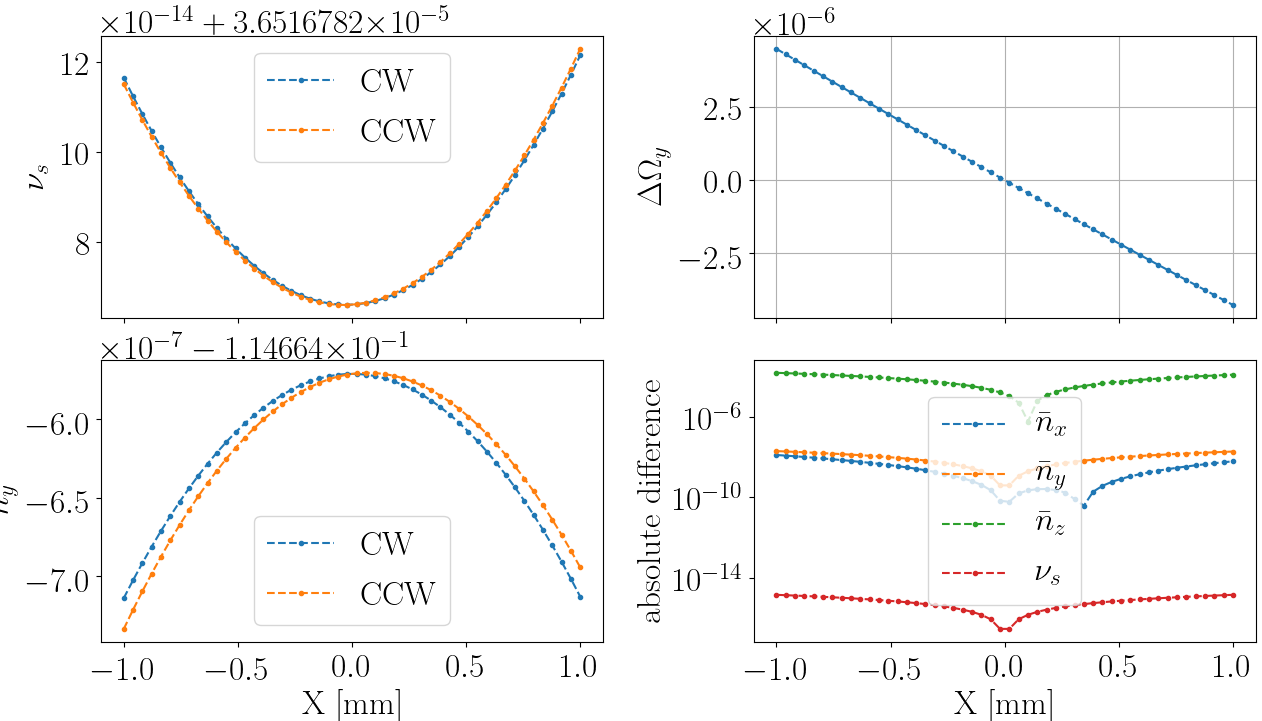
\includegraphics[width=\linewidth]{images/GFF/GFF_stune_range_X}}
  \subbottom[Разница между радиальными компонентами частоты прецессии CW и CCW пучков
против разницы вертикальных компонент (калибровочный график)\label{fig:X:calib_plot:omegas}]{%
    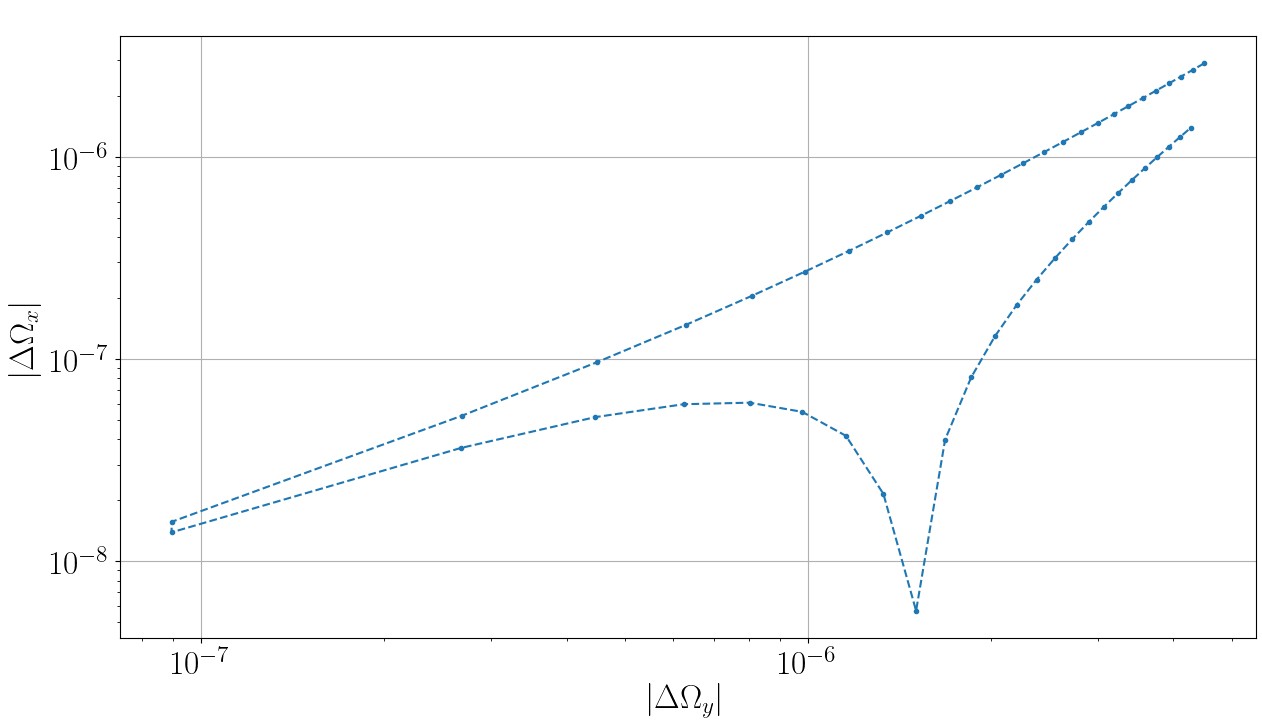
\includegraphics[width=\linewidth]{images/GFF/GFF_omegas_range_X}}
  \caption{Результаты симуляции для случая декогеренции, вызванной
    бетатронным движением в горизонтальной плоскости\label{fig:X:calib_plot}}
\end{figure}

\begin{figure}[h]
  \centering
  \subbottom[Зависимости спин-тюна и оси стабильного спина от вертикального смещения частицы
  от референсной орбиты\label{fig:Y:calib_plot:stune}]{%
    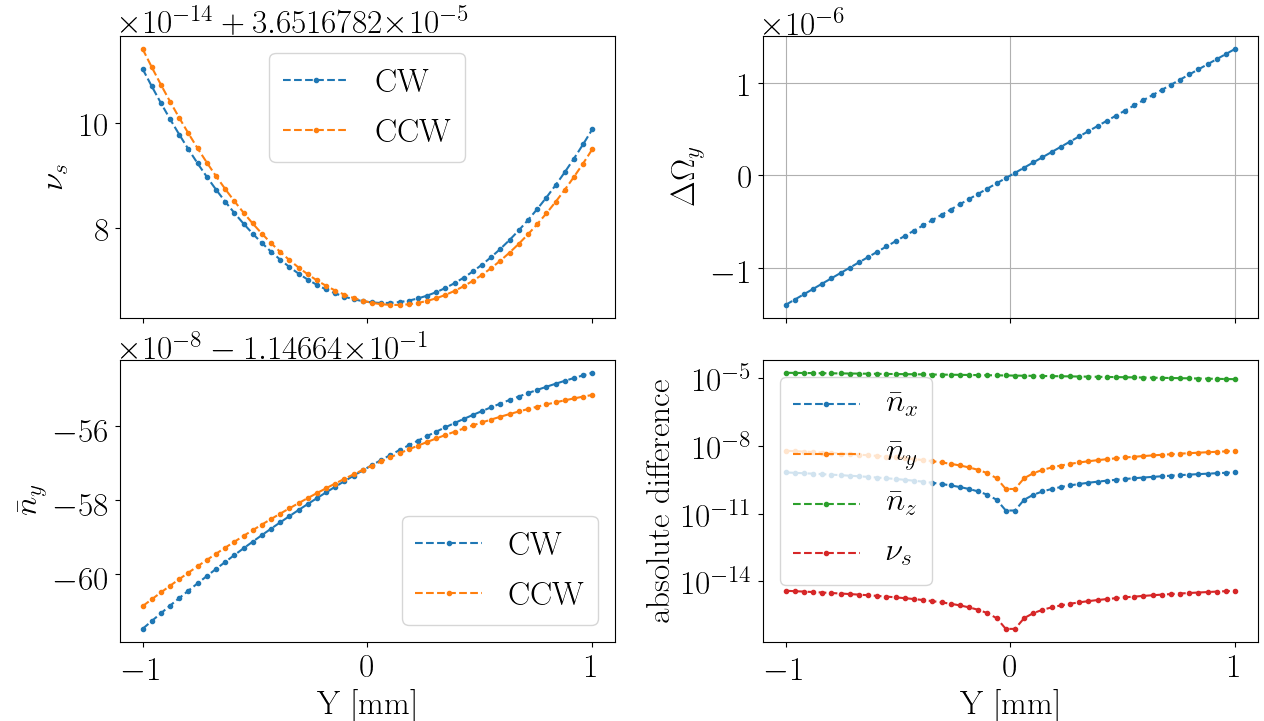
\includegraphics[width=\linewidth]{images/GFF/GFF_stune_range_Y}}
   \subbottom[Разница между радиальными компонентами частоты прецессии CW и CCW пучков
   против разницы вертикальных компонент (калибровочный график)\label{fig:Y:calib_plot:omegas}]{%
    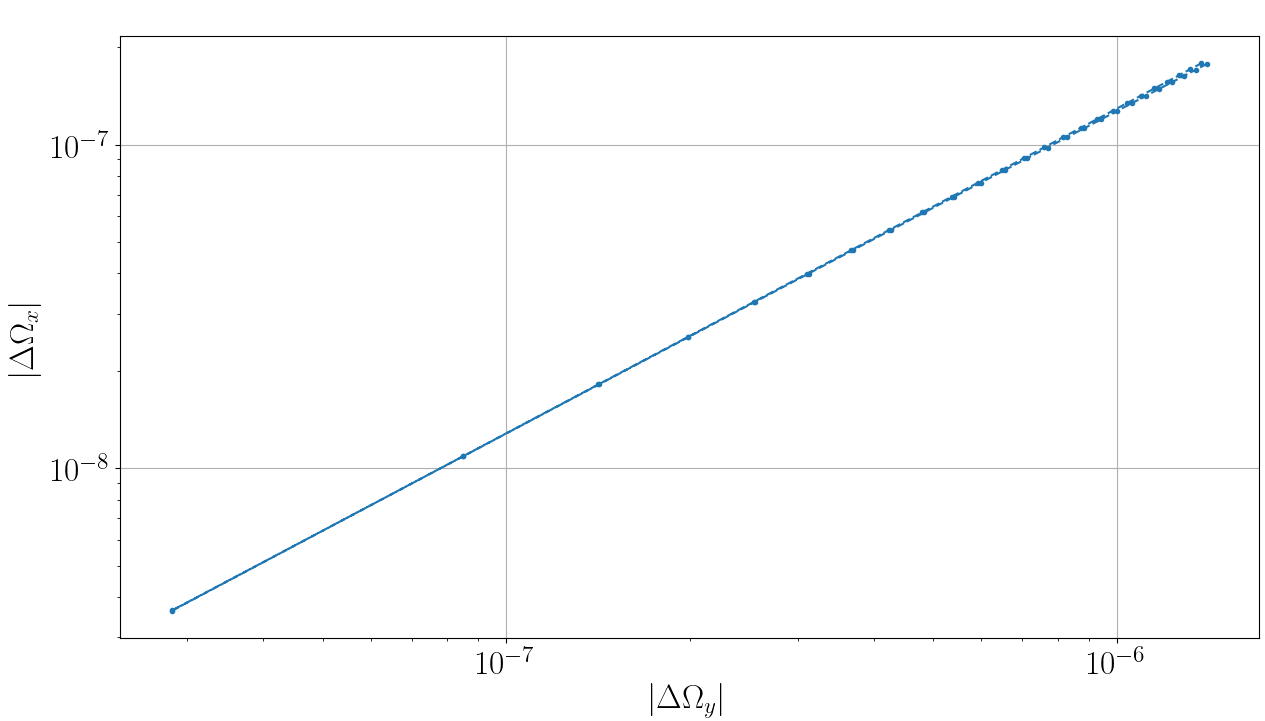
\includegraphics[width=\linewidth]{images/GFF/GFF_omegas_range_Y}}
  \caption{Результаты симуляции для случая декогеренции, вызванной
    бетатронным движением в вертикальной плоскости\label{fig:Y:calib_plot}}
\end{figure}

\begin{figure}[h]
  \centering
  \subbottom[Зависимости спин-тюна и оси стабильного спина от энергетического сдвига
  частицы от референсной энергии\label{fig:D:calib_plot:stune}]{%
    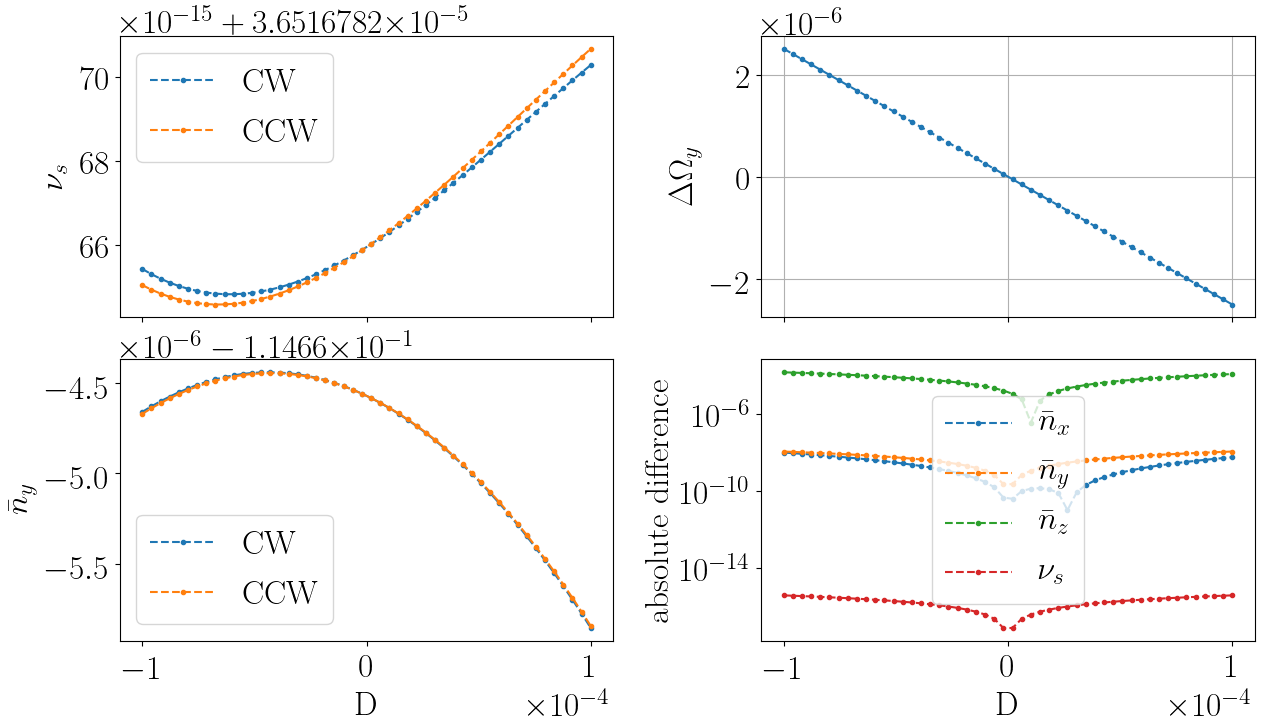
\includegraphics[width=\linewidth]{images/GFF/GFF_stune_range_D}}
  \subbottom[Разница между радиальными компонентами частоты прецессии CW и CCW пучков
  против разницы вертикальных компонент (калибровочный график)\label{fig:D:calib_plot:omegas}]{%
    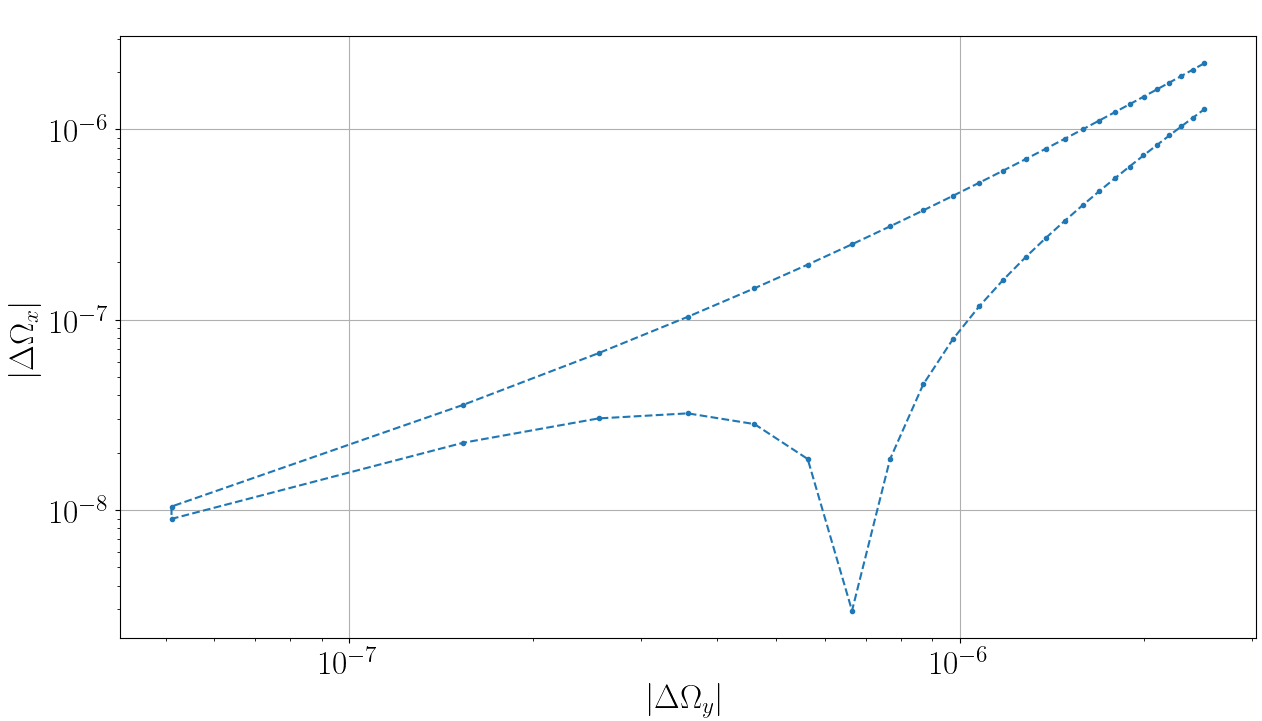
\includegraphics[width=\linewidth]{images/GFF/GFF_omegas_range_D}}
  \caption{Результаты симуляции для случая декогеренции, вызванной
    синхротронным движением\label{fig:D:calib_plot}}
\end{figure}
